% For PRD: \documentclass[aps,prd,twocolumn,superscriptaddress,nofootinbib]{revtex4-2}
\documentclass[10pt,twocolumn]{article}
\usepackage[a4paper,margin=1.9cm,columnsep=0.7cm]{geometry}
\usepackage{amsmath,amssymb}
\usepackage{booktabs,multirow}
\usepackage{graphicx}
\usepackage[numbers,sort&compress]{natbib}
\usepackage[hidelinks]{hyperref}
\usepackage{xcolor}
\newenvironment{acknowledgments}{\section*{Acknowledgments}}{}
\newcommand{\Bc}{B_c}
\newcommand{\Bcs}{B_c^*}
\newcommand{\cc}{c\bar c}
\newcommand{\bb}{b\bar b}
\newcommand{\cb}{c\bar b}
\newcommand{\MeV}{\,\mathrm{MeV}}
\newcommand{\GeV}{\,\mathrm{GeV}}
\newcommand{\GeVi}{\,\mathrm{GeV}^{-1}}
\graphicspath{{figures/}}

\begin{document}

\twocolumn[
\begin{@twocolumnfalse}
\begin{center}
{\LARGE\bfseries The heavy-quarkonium hyperfine splittings as the arbiter of the contact interaction}

\vspace{10pt}
{\large Peter Agyemang Oppong}

\vspace{2pt}
{\small\itshape School of Physics and Astronomy, University of Glasgow, Glasgow G12 8QQ, United Kingdom}

\vspace{2pt}
{\small \today}
\end{center}
\begin{quote}\small
With the ATLAS measurement of the $\Bcs$ mass, every $S$-wave hyperfine splitting of the $\cc$, $\bb$ and $\cb$ ground and first-excited states is now known, together with the $P$-wave singlet--triplet offsets of $h_c$, $h_b(1P)$ and $h_b(2P)$: nine observables that test the spin--spin interaction of a heavy quark and antiquark across three reduced masses and two radial excitations.
We confront them with four prescriptions for the contact term---first-order perturbation theory, a mass-independent Gaussian smearing, the mass-dependent smearing of Godfrey and Isgur, and a Yukawa form factor with the mass scale of the lattice spin--spin potential---each with a fixed or a one-loop running coupling, on top of a spin-averaged potential and quark masses fixed beforehand by the spin-independent spectrum, so that nothing but the contact prescription is tested.
The data are decisive on three points.
The $h_c$, which sits at the $\chi_{cJ}$ centroid to $0.2\MeV$, limits the r.m.s.\ radius of any smearing to below $0.07\,$fm, an order of magnitude smaller than the widths used in standard potential models and small enough that smearing has no effect the data can see.
The $\cc$/$\bb$ ratio of the $1S$ splittings, together with the $2S/1S$ ratios, fixes the short-distance strength $\kappa$ of the Coulomb term, to which the spin-averaged spectrum is blind: with a running coupling the splittings require $\kappa\simeq0.2$--$0.4$, consistent with $\tfrac43\alpha_s$, whereas with a fixed coupling they require $\kappa=0$.
And every prescription fails in the same place: the charmonium $2S$ splitting is predicted at $55$--$63\MeV$ against the measured $48.3$, the one state among the nine for which coupled-channel shifts of this size have been computed.
With that state removed, first-order perturbation theory with a running coupling and no smearing describes the other eight with $\chi^2=2.6$ for seven degrees of freedom and a single parameter, $\Lambda=0.21\GeV$; the smeared forms, with two or three parameters, reach $\chi^2/\mathrm{dof}=1.1$--$2.1$.
Fitted to charmonium and bottomonium alone, the prescriptions separate only in what they predict for $\Bc$: first-order with running coupling gives $M(\Bcs)-M(\Bc)=62\pm2\MeV$ ($64.5$ with the annihilation-corrected charmonium input) and $M(\Bcs(2S))-M(\Bc(2S))=33\pm1\MeV$, the smeared forms $50$--$58\MeV$ and $26$--$30\MeV$.
The ATLAS value, $64.5\pm1.8\MeV$, selects the first; the lattice values, $54(3)$ and $55(3)\MeV$, would select the second.
The $\Bc$ hyperfine splitting is therefore the arbiter between contact prescriptions, and experiment and lattice QCD currently point to different ones.
\end{quote}
\vspace{6pt}
\end{@twocolumnfalse}
]

% ===========================================================================
\section{Introduction}
\label{sec:intro}

The spin--spin interaction between a heavy quark and antiquark is, at leading order, a contact term: one-gluon exchange gives
\begin{equation}
  H_{SS}=\frac{32\pi\alpha_s}{9\,m_1m_2}\,\mathbf s_1\!\cdot\!\mathbf s_2\,\delta^3(\mathbf r),
  \label{eq:hss}
\end{equation}
so that the $S$-wave hyperfine splitting is proportional to $|\psi(0)|^2/m_1m_2$ and the $P$-wave singlet sits at the triplet centroid.
In first-order perturbation theory this works tolerably for charmonium and bottomonium separately but has always been in tension between them~\cite{Eichten1994,Godfrey1985}, and because a $\delta$ function is singular when inserted into a Schrödinger equation, most potential models replace it by a smeared version, Gaussian with a width of order $1\GeV$~\cite{Godfrey1985,BGS2005}, and solve the singlet and triplet non-perturbatively.
The width is then a parameter, mass-independent in some models and mass-dependent in others, and its value has been set by the charmonium $1S$ splitting alone.

Until recently the data could not arbitrate.
What has changed is that the $\Bcs$ has been found~\cite{ATLAS2026}, giving a third reduced mass; the $\Bc(2S)$ doublet has been resolved~\cite{CMS2019,LHCb2019}; the $\eta_b(2S)$ exists; and the $h_c$ and $h_b$ masses are known to $0.1$--$1\MeV$.
Nine hyperfine observables are now measured (Table~\ref{tab:data}), spanning reduced masses from $0.9$ to $2.6\GeV$ and two radial excitations, and they test the mass dependence, the radial dependence and the range of the contact interaction independently.
Two of them deserve a caveat.
The $\eta_b(2S)$ rests on a single Belle observation~\cite{PDG2026} that is omitted from the PDG summary table and was not confirmed in a later Belle search; we use it with its full, symmetrised error ($\pm4.2\MeV$) and check that nothing depends on it.
The $\Bc(2S)$ splitting is not measured directly: CMS and LHCb see the $\Bcs(2S)$ only through its decay to $\Bcs\gamma$ with the photon unreconstructed, so the observed $29.1\pm1.7\MeV$ separation of the two $2S$ peaks~\cite{CMS2019} is $\Delta_{1S}-\Delta_{2S}$, and $\Delta_{2S}=35.4\pm2.5\MeV$ follows only when combined with the ATLAS $\Delta_{1S}$.
This paper asks what they say.

The question is only sharp if nothing else is being fitted.
We therefore take the spin-averaged potential $V(r)$ and the quark masses from a model-independent extraction from the spin-averaged $\cc+\bb$ spectrum~\cite{Oppong2026b}, hold them fixed, and fit only the one to three parameters of each contact prescription to the nine splittings.
Section~\ref{sec:method} sets this up, Sec.~\ref{sec:results} gives the comparison, Sec.~\ref{sec:bc} the consequences for $\Bc$, and Sec.~\ref{sec:conclusions} concludes.

% ===========================================================================
\section{Set-up}
\label{sec:method}

\begin{table}[t]
\caption{The hyperfine data (MeV)~\cite{PDG2026,ATLAS2026,CMS2019}. $S$ waves: $M(^3S_1)-M(^1S_0)$. $P$ waves: $M(^1P_1)$ minus the $(2J+1)$-weighted centroid of the $^3P_J$ triplet, which vanishes for a pure contact term. Theory floors of $3\MeV$ ($S$) and $0.5\MeV$ ($P$) are added in quadrature in the fits.}
\label{tab:data}
\centering\footnotesize
\begin{tabular}{lcl}
\toprule
observable & value & source \\
\midrule
$c\bar c\,1S$ & $112.81\pm0.30$ & $J/\psi-\eta_c$ \\
$c\bar c\,2S$ & $48.30\pm0.60$ & $\psi(2S)-\eta_c(2S)$ \\
$b\bar b\,1S$ & $61.70\pm2.00$ & $\Upsilon(1S)-\eta_b$ \\
$b\bar b\,2S$ & $24.40\pm3.50$ & $\Upsilon(2S)-\eta_b(2S)$ (Belle) \\
$B_c\,1S$ & $64.50\pm1.70$ & $\Bcs-\Bc$, ATLAS \\
$B_c\,2S$ & $35.40\pm2.40$ & $\Bcs(2S)-\Bc(2S)$, ATLAS$+$CMS \\
$h_c$ & $0.07\pm0.15$ & $h_c-\bar M(\chi_{cJ})$ \\
$h_b(1P)$ & $-0.57\pm0.80$ & $h_b(1P)-\bar M(\chi_{bJ}(1P))$ \\
$h_b(2P)$ & $-0.44\pm1.20$ & $h_b(2P)-\bar M(\chi_{bJ}(2P))$ \\
\bottomrule

\end{tabular}
\end{table}

\paragraph{Spin-averaged potential.}
Reference~\cite{Oppong2026b} represents $V(r)=-\kappa/r+S(r)$, $S$ a cubic spline, and fits it with $m_c$ and $m_b$ to the eleven spin-averaged $\cc$ and $\bb$ multiplet centroids.
The spectrum determines $S(r)$ to $40$--$70\MeV$ for $0.7\le r\le7\GeVi$ but is blind to the Coulomb coefficient: fits at $\kappa=0$, $0.2$, $0.4$, $0.6$ and $0.8$ have $\chi^2=12.0$--$12.2$ for the same eleven centroids, with $m_c=1.78$--$1.81$ and $m_b=5.16$--$5.18\GeV$.
These five potentials, each with its own masses, are the fixed input here, and $\kappa$ is the one property of $V(r)$ that the hyperfine data, which probe $|\psi(0)|^2$, are in a position to decide.

\paragraph{Prescriptions.}
All four have the structure of Eq.~\eqref{eq:hss} with $\delta^3(\mathbf r)$ replaced by a normalised profile $\delta_X(r)$:
\begin{itemize}
\item \emph{first-order}: $\delta_X=\delta^3$, the splitting evaluated in first-order perturbation theory, $\Delta=8\alpha_s|R(0)|^2/9m_1m_2$; no $P$-wave shift. No free parameter beyond the coupling.
\item \emph{Gaussian}: $\delta_X=(\sigma/\sqrt\pi)^3e^{-\sigma^2r^2}$, one width for all systems, as in Ref.~\cite{BGS2005}. One parameter, $\sigma$.
\item \emph{Godfrey--Isgur}: a Gaussian whose width depends on the quark masses, $\sigma_{ij}^2=\sigma_0^2\big[\tfrac12+\tfrac12\big(\tfrac{4m_im_j}{(m_i+m_j)^2}\big)^4\big]+s^2\big(\tfrac{2m_im_j}{m_i+m_j}\big)^2$~\cite{Godfrey1985}. Two parameters, $\sigma_0$ and $s$.
\item \emph{Yukawa}: $\delta_X=m^2e^{-mr}/4\pi r$. This is the functional form with which Koma and Koma fit the non-perturbative part of the lattice spin--spin potential~\cite{KomaKoma2007}, with $m$ the $0^{-+}$ glueball mass, $2.47\GeV$; we use it as a one-parameter alternative to the Gaussian shape, with $m$ free and $m=2.47\GeV$ as a check, and do not claim more lattice content for it than that.
\end{itemize}
For the three smeared forms the singlet ($\mathbf s_1\!\cdot\!\mathbf s_2=-\tfrac34$) and triplet ($+\tfrac14$) radial equations are solved non-perturbatively, for $S$ and $P$ waves alike, with the Numerov method of Ref.~\cite{Oppong2026}; the $P$-wave observable is then the singlet energy minus the triplet one, the spin--orbit and tensor terms cancelling in the centroid.
The coupling is either one value $\alpha_s$ for all three systems (``fixed'') or the one-loop running coupling at $\mu=\sqrt{m_1m_2}$ with $\Lambda$ fitted (``running''), which makes $\alpha_s(\bb)/\alpha_s(\cc)\simeq0.68$.
Each prescription is fitted at each $\kappa$; fits with the $\cc$ $2S$ splitting removed, and with theory floors of $1$ and $5\MeV$, are the variants.
Propagated errors are scaled by $\sqrt{\chi^2/\mathrm{dof}}$ where that exceeds one.

% ===========================================================================
\section{What the data decide}
\label{sec:results}

\begin{figure*}[t]
\centering
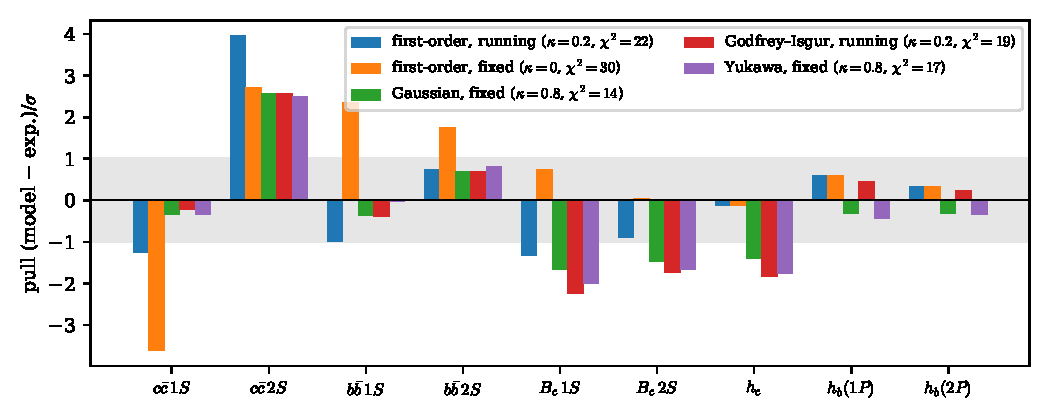
\includegraphics[width=0.95\textwidth]{fig1_pulls}
\caption{Pulls of the nine hyperfine observables for each prescription at the Coulomb strength $\kappa$ that suits it best (Table~\ref{tab:main}). The grey band is $\pm1\sigma$. Every prescription over-predicts the $\cc$ $2S$ splitting.}
\label{fig:pulls}
\end{figure*}

\begin{table*}[t]
\caption{The four prescriptions with fixed and running coupling, each at the $\kappa$ of Table~\ref{tab:kscan} that minimises its $\chi^2$: fit quality for the nine observables, fitted parameters (GeV), and the r.m.s.\ radius of the contact term for $\cc$ (and $\bb$ where it differs). Errors scaled by $\sqrt{\chi^2/\mathrm{dof}}$.}
\label{tab:main}
\centering\small
\begin{tabular}{llcclc}
\toprule
prescription & $\alpha_s$ & $\kappa$ & $\chi^2/\mathrm{dof}$ & parameters & r.m.s.\ radius [fm] \\
\midrule
first-order & running & 0.2 & 22.1/8 & $\Lambda=0.19\pm0.01$ & -- \\
first-order & fixed & 0 & 30.9/8 & $\alpha_s=0.33\pm0.01$ & -- \\
Gaussian & fixed & 0.8 & 14.8/7 & $\alpha_s=0.28\pm0.03$, $\sigma=4.35\pm0.77$ & 0.056 \\
Gaussian & running & 0 & 102.9/7 & $\Lambda=0.12\pm0.05$, $\sigma=4.83\pm1.40$ & 0.050 \\
Godfrey--Isgur & running & 0.2 & 19.2/6 & $\Lambda=0.15\pm0.05$, $\sigma_0=0.20\pm8.98$, $s=2.16\pm0.63$ & 0.062 / 0.022 \\
Godfrey--Isgur & fixed & 0 & 17.4/6 & $\alpha_s=0.28\pm0.04$, $\sigma_0=3.81\pm0.88$, $s=1.42\pm0.75$ & 0.053 / 0.029 \\
Yukawa & fixed & 0.8 & 17.5/7 & $\alpha_s=0.27\pm0.03$, $m=6.97\pm1.32$ & 0.069 \\
Yukawa & running & 0 & 116.0/7 & $\Lambda=0.12\pm0.04$, $m=7.59\pm1.88$ & 0.064 \\
\bottomrule

\end{tabular}
\end{table*}

\begin{table*}[t]
\caption{Predicted splittings (MeV) for the fits of Table~\ref{tab:main}, in the order of that table.}
\label{tab:pred}
\centering\small
\setlength{\tabcolsep}{4pt}
\begin{tabular}{lccccccccc}
\toprule
 & $c\bar c\,1S$ & $c\bar c\,2S$ & $b\bar b\,1S$ & $b\bar b\,2S$ & $B_c\,1S$ & $B_c\,2S$ & $h_c$ & $h_b(1P)$ & $h_b(2P)$ \\
\midrule
experiment & $112.8\pm0.3$ & $48.3\pm0.6$ & $61.7\pm2.0$ & $24.4\pm3.5$ & $64.5\pm1.7$ & $35.4\pm2.4$ & $0.1\pm0.1$ & $-0.6\pm0.8$ & $-0.4\pm1.2$ \\
\midrule
first-order, running & 109.0 & 60.4 & 58.2 & 28.2 & 59.9 & 31.9 & 0.0 & 0.0 & 0.0 \\
first-order, fixed & 101.8 & 56.5 & 70.1 & 33.4 & 67.0 & 35.5 & 0.0 & 0.0 & 0.0 \\
Gaussian, fixed & 111.8 & 56.2 & 60.3 & 27.9 & 58.7 & 29.6 & -0.7 & -0.9 & -0.9 \\
Gaussian, running & 115.5 & 58.5 & 36.0 & 15.8 & 47.0 & 23.5 & -0.6 & -0.6 & -0.6 \\
Godfrey--Isgur, running & 112.1 & 56.1 & 60.3 & 28.0 & 56.7 & 28.6 & -0.9 & -0.1 & -0.1 \\
Godfrey--Isgur, fixed & 110.3 & 55.9 & 65.7 & 29.6 & 58.1 & 28.9 & -0.6 & -0.3 & -0.3 \\
Yukawa, fixed & 111.8 & 55.9 & 61.5 & 28.6 & 57.6 & 28.9 & -0.9 & -1.0 & -0.9 \\
Yukawa, running & 115.5 & 58.1 & 34.5 & 15.0 & 45.6 & 22.6 & -0.8 & -0.7 & -0.7 \\
\bottomrule

\end{tabular}
\end{table*}

Tables~\ref{tab:main} and \ref{tab:pred} and Fig.~\ref{fig:pulls} summarise the fits.
No prescription describes all nine observables: the best $\chi^2$ is $15$--$22$ for six to eight degrees of freedom, and the pattern of pulls is the same for all of them.
Three features of the data account for this, and each settles a question.

\paragraph{The $h_c$ excludes any visible smearing.}
A smeared contact term shifts $P$-wave singlets below the triplet centroid by $\langle\delta_X\rangle_{P}$, which grows with the width: the $h_c$ is predicted $16\MeV$ below the $\chi_{cJ}$ centroid for $\sigma=1\GeV$ and $4\MeV$ below for $\sigma=2\GeV$, with $\alpha_s$ in each case tuned to the $\cc$ $1S$ datum (Table~\ref{tab:pwave}, Fig.~\ref{fig:pwave}).
The measured offset is $+0.07\pm0.15\MeV$; that it is consistent with zero, as a pure contact interaction requires, was noted when CLEO first measured the $h_c$ mass precisely~\cite{CLEO2008}, and what follows is the quantitative version.
Smearing widths of $\sigma\simeq1$--$1.2\GeV$, which are what Refs.~\cite{BGS2005} and the charmonium literature use and which predict $h_c$ masses of $3516$--$3517\MeV$, are excluded by two orders of magnitude; the data allow a r.m.s.\ radius below about $0.07\,$fm ($\sigma\gtrsim3.5\GeV$), the $\sigma=3\GeV$ offset of $-1.6\MeV$ being $3\sigma$ away even with the $0.5\MeV$ theory floor.
Every fit in Table~\ref{tab:main} finds this on its own: the Gaussian and Yukawa widths run to $\sigma=4.3$--$4.8\GeV$ and $m=7$--$8\GeV$, radii of $0.05$--$0.07\,$fm, where the profile is narrower than any feature of the wave functions (Fig.~\ref{fig:profiles}).
The lattice scale $m=2.47\GeV$ is excluded for the same reason ($h_c$ at $-5\MeV$).
The widths do not run further for a reason worth stating: a $\delta$ function has no non-perturbative solution in three dimensions, the attractive singlet channel collapsing as the width shrinks, so the smeared prescriptions have no first-order limit.
At $\sigma=4\GeV$ the non-perturbative $\cc$ $1S$ splitting is already $25\%$ above first order for the same $\alpha_s$ and the $\bb$ one $20\%$ below it; at $\sigma=8\GeV$ the $\cc$ ratio is $3$ and at $16\GeV$ it is $260$.
The fitted widths sit at the edge of this regime, and what the fits with smearing are really doing is using the onset of the collapse as a free parameter.
Smearing, in short, is not something the data can see; it is a regulator, and the hyperfine splittings tell us to remove it.

\begin{table}[t]
\caption{Gaussian contact term of width $\sigma$ with $\alpha_s$ tuned to reproduce the $\cc$ $1S$ splitting ($\kappa=0.4$): the predicted $\cc$ $2S$ splitting and $h_c$ offset (MeV). Measured: $48.3$ and $+0.07\pm0.15$.}
\label{tab:pwave}
\centering\small
\begin{tabular}{ccccc}
\toprule
$\sigma$ [GeV] & r.m.s.\ [fm] & $\alpha_s$ & $c\bar c\,2S$ & $M(h_c)-\bar M(\chi_{cJ})$ \\
\midrule
0.5 & 0.483 & 2.78 & 33.6 & $-46.33$ \\
0.7 & 0.345 & 1.50 & 33.6 & $-29.29$ \\
1 & 0.242 & 0.89 & 39.6 & $-16.05$ \\
1.5 & 0.161 & 0.58 & 47.2 & $-7.28$ \\
2 & 0.121 & 0.45 & 51.3 & $-3.97$ \\
3 & 0.081 & 0.35 & 55.0 & $-1.62$ \\
4 & 0.060 & 0.30 & 56.4 & $-0.84$ \\
5 & 0.048 & 0.26 & 56.4 & $-0.49$ \\
\bottomrule

\end{tabular}
\end{table}

\begin{figure}[t]
\centering
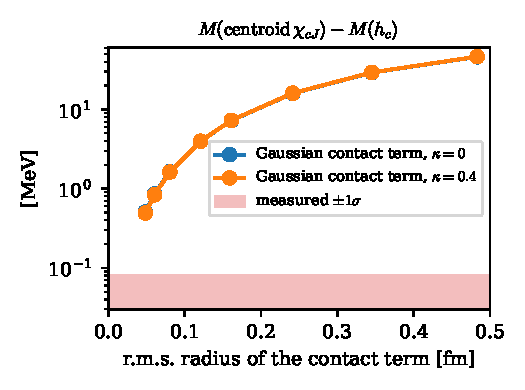
\includegraphics[width=\columnwidth]{fig3_pwave_bound}
\caption{The $h_c$ offset below the $\chi_{cJ}$ centroid produced by a Gaussian contact term, as a function of its r.m.s.\ radius, with $\alpha_s$ tuned to the $\cc$ $1S$ splitting; the band is the measurement.}
\label{fig:pwave}
\end{figure}

\begin{figure}[t]
\centering
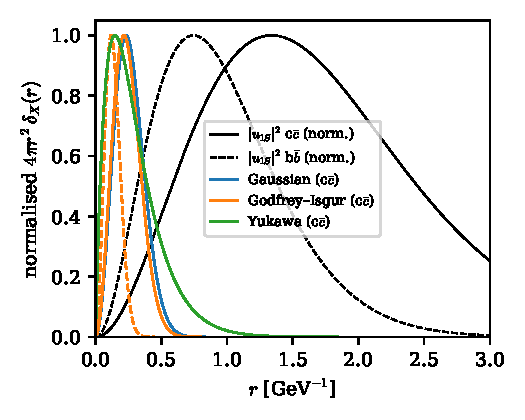
\includegraphics[width=\columnwidth]{fig2_profiles}
\caption{The fitted contact-term profiles $4\pi r^2\delta_X(r)$ (fixed coupling, $\kappa=0$) compared with the $1S$ wave functions. The fitted widths are far inside the wave functions.}
\label{fig:profiles}
\end{figure}

\paragraph{The $\cc$/$\bb$ ratio fixes the Coulomb strength, given the running.}
The ratio of the $\bb$ to the $\cc$ $1S$ splitting, $0.547\pm0.018$, is $|R_{\bb}(0)|^2m_c^2\alpha_s(\bb)/|R_{\cc}(0)|^2m_b^2\alpha_s(\cc)$ in first order, and $|R(0)|^2$ for the heavier system grows faster with $\kappa$.
Table~\ref{tab:kscan} and Fig.~\ref{fig:kscan} show the $\chi^2$ of each prescription against the five values of $\kappa$ the spectrum allows.
With a fixed coupling, first-order perturbation theory wants $\kappa=0$---no Coulomb term at all---and is excluded at any $\kappa\ge0.2$ ($\chi^2\ge53$); with the running coupling, whose $\alpha_s(\bb)/\alpha_s(\cc)=0.68$ supplies two-thirds of the mass dependence, it wants $\kappa=0.2$--$0.4$ and is excluded at $\kappa\ge0.6$.
That range is $\tfrac43\alpha_s$ for $\alpha_s=0.15$--$0.3$, the one-gluon-exchange value, which the fixed-coupling fit cannot accommodate.
The smeared prescriptions with a fixed coupling do the opposite, preferring $\kappa\ge0.6$, because the non-perturbative response to the near-$\delta$ term, which enhances $\cc$ and reduces $\bb$, supplies mass dependence of the wrong sign that a stronger Coulomb term must undo; with a running coupling the mass-independent Gaussian and Yukawa forms fail at every $\kappa$ ($\chi^2\ge80$), since both effects then act in the same direction on $\bb$, while the Godfrey--Isgur form survives by making its width mass-dependent ($s\simeq2$), which is to say by putting the mass dependence back by hand.
The short-distance strength of the potential and the running of the coupling are therefore not separately determined by the hyperfine data; they are determined together, and the physically motivated combination---$\kappa\simeq\tfrac43\alpha_s$ with $\alpha_s$ running---is the one the data accept.
The preference does not depend on the theory floor: with $5\MeV$ instead of $3$ the first-order $\chi^2$ runs $13.8$, $8.8$, $9.7$, $18.9$, $39.3$ over $\kappa=0$--$0.8$ with the running coupling and $12.5$, $22.6$, $39.5$, $64.5$, $98.2$ with the fixed one (Table~\ref{tab:kscan}, lower block).

\begin{table}[t]
\caption{$\chi^2$ of each prescription (nine observables) against the Coulomb strength $\kappa$ of the spin-averaged potential; lower block, the first-order fits with a $5\MeV$ theory floor. The spin-averaged spectrum has $\chi^2=12.0$--$12.2$ at every $\kappa$.}
\label{tab:kscan}
\centering\footnotesize
\setlength{\tabcolsep}{3pt}
\begin{tabular}{llccccc}
\toprule
prescription & $\alpha_s$ & $\kappa=0$ & $0.2$ & $0.4$ & $0.6$ & $0.8$ \\
\midrule
first-order & running & 33.6 & 21.8 & 22.8 & 42.2 & 86.9 \\
first-order & fixed & 30.1 & 53.0 & 92.0 & 150.7 & 231.6 \\
Gaussian & fixed & 26.9 & 22.5 & 18.8 & 16.0 & 14.5 \\
Gaussian & running & 101.1 & -- & 80.9 & -- & -- \\
Godfrey--Isgur & running & 25.3 & 18.9 & 21.0 & 27.9 & 34.7 \\
Godfrey--Isgur & fixed & 17.0 & -- & 22.9 & -- & -- \\
Yukawa & fixed & 34.3 & 28.1 & 22.8 & 18.8 & 17.1 \\
Yukawa & running & 113.9 & -- & 89.6 & -- & -- \\
\midrule

first-order, floor $5\MeV$ & running & 13.8 & 8.8 & 9.7 & 18.9 & 39.3 \\
first-order, floor $5\MeV$ & fixed & 12.5 & 22.6 & 39.5 & 64.5 & 98.2 \\
\bottomrule

\end{tabular}
\end{table}

\begin{figure}[t]
\centering
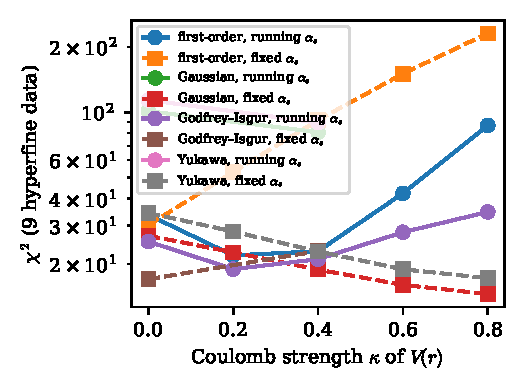
\includegraphics[width=\columnwidth]{fig4_kappa_scan}
\caption{The $\chi^2$ of Table~\ref{tab:kscan} against $\kappa$. Circles and solid lines: running coupling; squares and dashed lines: fixed.}
\label{fig:kscan}
\end{figure}

\paragraph{The $\cc$ $2S$ splitting is the universal outlier.}
Every fit in Table~\ref{tab:pred} predicts the $\psi(2S)$--$\eta_c(2S)$ splitting at $55$--$63\MeV$ against the measured $48.3\pm0.6$, and every $\cc$ $2S/1S$ ratio comes out $0.50$--$0.55$ against $0.43$.
This is not a failure the contact prescription can fix: the ratio is set by $|R_{2S}(0)|^2/|R_{1S}(0)|^2$, which the spin-averaged potential determines, and by second-order effects that are small for any profile the $h_c$ allows.
The $\bb$ ratio, $0.40\pm0.07$, and the $\Bc$ ratio, $0.55\pm0.04$, are both reproduced (predicted $0.46$--$0.49$ and $0.49$--$0.53$), and the lattice $\bb$ ratio, $0.445\pm0.028$~\cite{Dowdall2014}, agrees with the fits better than the experimental one does; the lattice $\bb$ $1S$ splitting itself, $57.5\pm2.5\MeV$~\cite{Hatton2021}, is $1.3\sigma$ below experiment and $1\sigma$ from the $\kappa=0.2$ fits.
The $\cc$ $2S$ states are the only ones among the nine within $50\MeV$ of an open-flavour threshold, and Eichten, Lane and Quigg~\cite{ELQ2004} computed the coupled-channel shifts for exactly these two: $+15.7\MeV$ for the $\eta_c(2S)$ and $-5.2\MeV$ for the $\psi(2S)$, reducing their splitting by $20.9\MeV$.
Our $12$--$15\MeV$ excess is that effect.
We therefore treat the $\cc$ $2S$ splitting as a coupled-channel observable rather than a contact-term one, and refit without it.

\paragraph{One parameter describes the rest.}
With the $\cc$ $2S$ removed, first-order perturbation theory with the running coupling fits the remaining eight observables with $\chi^2=2.6$ for seven degrees of freedom at $\kappa=0.2$ ($8.1$ at $\kappa=0.4$), with one parameter, $\Lambda=0.213\pm0.011\GeV$, i.e.\ $\alpha_s(\cc)=0.35$, $\alpha_s(\bb)=0.24$, $\alpha_s(\cb)=0.29$ (Table~\ref{tab:bc}).
Dropping the unconfirmed $\eta_b(2S)$ as well changes $\Lambda$ by $0.001\GeV$.
The smeared forms do less well with more parameters: $\chi^2/\mathrm{dof}=6.6/6$ (Gaussian), $9.7/6$ (Yukawa) and $10.7/5$ (Godfrey--Isgur), the excess coming entirely from the two $\Bc$ splittings, which they under-predict by $5$--$7\MeV$.
That is the one place where the prescriptions differ in what they say, and Sec.~\ref{sec:bc} turns it into a test.
One more correction is known and is not in any potential model: the $\eta_c$ annihilation shift.
The lattice value of the $\cc$ $1S$ splitting for the connected contribution alone is $120.3\pm1.1\MeV$~\cite{Hatton2020}, the difference from experiment being the $\eta_c\to gg$ shift of $7.3\pm1.2\MeV$.
A contact term compared with experiment is therefore being asked to reproduce $7\MeV$ of annihilation physics, and the right comparison for it is the connected value.
Fitting to $120.1\pm1.2$ instead of $112.8$ gives $\chi^2=2.1/7$ with $\Lambda=0.236\pm0.011\GeV$ (last row of Table~\ref{tab:bc}); the $\bb$ splittings are unchanged and the $\Bc$ ones move up by $2$--$3\MeV$.

% ===========================================================================
\section{The $\Bc$ hyperfine splittings}
\label{sec:bc}

\begin{table*}[t]
\caption{$\Bc$ hyperfine splittings (MeV). Upper block (a): fits to the charmonium and bottomonium data only ($\cc$ $2S$ excluded), so that the $\Bc$ columns are predictions; lower block (b): the same fits including the two $\Bc$ splittings. Errors are the propagated fit errors scaled by $\sqrt{\chi^2/\mathrm{dof}}$. Experiment: $\Delta_{1S}=64.5\pm1.8$~\cite{ATLAS2026}, $\Delta_{2S}=35.4\pm2.5$ (ATLAS$+$CMS), $\Delta_{1S}-\Delta_{2S}=29.1\pm1.7$ (CMS~\cite{CMS2019}), $30.9$ (LHCb~\cite{LHCb2019}); lattice $\Delta_{1S}=54\pm3$~\cite{Dowdall2012}, $55\pm3$~\cite{Mathur2018}. The last two columns are the predicted $\cc$ $2S$ splitting and $\Bc$ $P$-wave offset.}
\label{tab:bc}
\centering\small
\begin{tabular}{lccccccc}
\toprule
fit & $\chi^2/\mathrm{dof}$ & $\Delta_{1S}$ & $\Delta_{2S}$ & $\Delta_{1S}-\Delta_{2S}$ & $M(\Bcs)$ & $c\bar c\,2S$ & $B_c\,1P$ \\
\midrule
first-order, running, $\kappa=0.2$ & 1.6/5 & $61.6\pm1.3$ & $32.8\pm0.7$ & $28.8\pm0.6$ & $6336.1$ & 62.7 & +0.0 \\
first-order, running, $\kappa=0.4$ & 7.7/5 & $62.8\pm1.6$ & $33.6\pm0.9$ & $29.2\pm0.8$ & $6337.3$ & 60.9 & +0.0 \\
first-order, running, $\kappa=0.2$, lattice $c\bar c\,1S$ & 1.7/5 & $64.5\pm1.3$ & $34.4\pm0.7$ & $30.2\pm0.6$ & $6339.0$ & 66.3 & +0.0 \\
Gaussian, fixed, $\kappa=0.8$ & 2.0/4 & $57.6\pm2.7$ & $29.5\pm0.9$ & $28.1\pm1.9$ & $6332.1$ & 57.0 & -0.3 \\
Yukawa, fixed, $\kappa=0.8$ & 1.5/4 & $50.0\pm4.8$ & $26.1\pm2.3$ & $23.8\pm2.6$ & $6324.5$ & 58.0 & -0.1 \\
Godfrey--Isgur, running, $\kappa=0.2$ & 1.6/3 & $52.5\pm9.4$ & $27.1\pm4.3$ & $25.4\pm5.1$ & $6327.0$ & 58.3 & -0.1 \\
\midrule
first-order, running, $\kappa=0.2$ & 2.6/7 & $62.1\pm1.2$ & $33.1\pm0.6$ & $29.0\pm0.5$ & $6336.6$ & 63.2 & +0.0 \\
first-order, running, $\kappa=0.4$ & 8.1/7 & $63.1\pm1.3$ & $33.8\pm0.7$ & $29.3\pm0.6$ & $6337.6$ & 61.3 & +0.0 \\
first-order, running, $\kappa=0.2$, lattice $c\bar c\,1S$ & 1.8/7 & $64.6\pm1.2$ & $34.4\pm0.6$ & $30.2\pm0.6$ & $6339.1$ & 66.4 & +0.0 \\
Gaussian, fixed, $\kappa=0.8$ & 6.6/6 & $59.5\pm1.7$ & $30.2\pm0.6$ & $29.4\pm1.3$ & $6334.0$ & 57.6 & -0.5 \\
Yukawa, fixed, $\kappa=0.8$ & 9.7/6 & $58.1\pm2.3$ & $29.3\pm0.7$ & $28.8\pm1.7$ & $6332.6$ & 57.4 & -0.6 \\
Godfrey--Isgur, running, $\kappa=0.2$ & 10.7/5 & $57.1\pm3.1$ & $29.0\pm1.5$ & $28.1\pm1.8$ & $6331.6$ & 58.0 & -0.2 \\
\bottomrule

\end{tabular}
\end{table*}

\begin{table}[t]
\caption{Shifts (MeV) of the first-order, running-coupling prediction for the $\Bc$ splittings (block (a) of Table~\ref{tab:bc}, $\kappa=0.2$) under the systematic variations considered. The quark-mass shifts are the $1\sigma$ errors of the centroid extraction with $V(r)$ held fixed.}
\label{tab:syst}
\centering\small
\begin{tabular}{lcc}
\toprule
variation & $\delta\Delta_{1S}$ & $\delta\Delta_{2S}$ \\
\midrule
$\kappa=0.4$ instead of $0.2$ & $+1.2$ & $+0.8$ \\
$m_c+0.024\GeV$ & $+0.6$ & $+0.3$ \\
$m_c-0.024\GeV$ & $-0.6$ & $-0.3$ \\
$m_b+0.023\GeV$ & $-0.2$ & $-0.1$ \\
$m_b-0.023\GeV$ & $+0.2$ & $+0.1$ \\
lattice (connected) $c\bar c\,1S$ input & $+2.9$ & $+1.5$ \\
\bottomrule

\end{tabular}
\end{table}

The $\Bc$ is the system where the prescriptions differ most, because it is the only one whose reduced mass is not used to set their parameters, and it is where experiment and lattice QCD disagree: ATLAS finds $M(\Bcs)-M(\Bc)=64.5\pm1.8\MeV$~\cite{ATLAS2026}, HPQCD predicted $54\pm3$~\cite{Dowdall2012} and Mathur, Padmanath and Mondal $55\pm3$~\cite{Mathur2018}, a $3\sigma$ difference.
To make a prediction rather than a fit, block (a) of Table~\ref{tab:bc} repeats each acceptable fit with the two $\Bc$ splittings removed from the data, so that its parameters are set by charmonium and bottomonium alone and the $\cb$ system is interpolated.
Every prescription then describes the six remaining equal-mass observables ($\chi^2/\mathrm{dof}\le0.5$); they are indistinguishable on $\cc$ and $\bb$ and differ only in $\Bc$.
First-order perturbation theory with the running coupling predicts $\Delta_{1S}=61.6\pm1.3$ at $\kappa=0.2$ and $62.8\pm1.6\MeV$ at $\kappa=0.4$, and $\Delta_{2S}=32.8$--$33.6\MeV$.
The smeared forms predict less, and with larger errors: $57.6\pm2.7$ (Gaussian), $52.5\pm9.4$ (Godfrey--Isgur) and $50.0\pm4.8\MeV$ (Yukawa) for $\Delta_{1S}$, because the non-perturbative enhancement of the singlet, which grows with the compactness of the wave function, is tuned away by the fit for $\cc$ and $\bb$ separately but not for the intermediate $\cb$ system.
Including the $\Bc$ data in the fit (block (b)) moves the first-order prediction by $0.5\MeV$ and pulls the smeared ones up by $2$--$8\MeV$ at the cost of their $\chi^2$.
Table~\ref{tab:syst} gives the remaining systematics of the first-order prediction: $\kappa$ within the range the data allow ($+1.2\MeV$), the quark masses ($\pm0.6$), and the $\eta_c$ annihilation correction to the charmonium input ($+2.9$).
Taking $\kappa=0.2$ with the measured inputs as central and adding the $\kappa$ and mass variations in quadrature,
\begin{align}
  M(\Bcs)-M(\Bc) &= 62\pm1\pm1\MeV, \\
  M(\Bcs(2S))-M(\Bc(2S)) &= 33\pm1\pm1\MeV, \\
  \Delta_{1S}-\Delta_{2S} &= 29\pm1\MeV,
\end{align}
or $64.5$, $34.4$ and $30\MeV$ with the annihilation-corrected charmonium input, against the measured $64.5\pm1.8$, $35.4\pm2.5$ and $29.1\pm1.7$.
The first-order prediction agrees with ATLAS at $1.3\sigma$ with the measured charmonium input and at $0.0\sigma$ with the annihilation-corrected one, and lies $2$--$3\sigma$ above the lattice values; the smeared predictions agree with the lattice and lie $2$--$3\sigma$ below ATLAS.
The $\Bc$ hyperfine splitting thus discriminates between contact prescriptions that the equal-mass systems cannot separate, and the measurement and the lattice at present select different ones.
If ATLAS stands, the contact interaction is the unsmeared one-gluon-exchange term with a running coupling; if the lattice value stands, the hyperfine data would be telling us that the non-perturbative singlet enhancement of a near-$\delta$ term is real physics rather than an artefact of the regulator, which would be surprising given Sec.~\ref{sec:results}.
A confirmation of the ATLAS $\Bcs$ by CMS or LHCb, or a lattice determination with the $\Bc$ at the few-MeV level of the current $\bb$ result~\cite{Hatton2021}, would settle it.
The $\Bc$ $P$-wave singlet--triplet offset is predicted to vanish to $0.5\MeV$ by every prescription.

% ===========================================================================
\section{Conclusions}
\label{sec:conclusions}

The nine measured heavy-quarkonium hyperfine observables, confronted with four contact-interaction prescriptions on top of a spin-averaged potential fixed by the spectrum, decide the following:
\begin{enumerate}
\item The $h_c$ offset from the $\chi_{cJ}$ centroid, $0.07\pm0.15\MeV$, limits the r.m.s.\ radius of any smeared contact term to below $0.07\,$fm. The $\sigma\simeq1\GeV$ Gaussians of the potential-model literature are excluded by two orders of magnitude, and the fits themselves push every smearing to the point where it is invisible.
\item With a one-loop running coupling, the $\cc$/$\bb$ hyperfine ratio selects a Coulomb strength $\kappa=0.2$--$0.4$ in the spin-averaged potential, consistent with $\tfrac43\alpha_s$ and invisible to the spectrum itself; with a fixed coupling it selects $\kappa=0$. Running and Coulomb strength are determined jointly, and only their one-gluon-exchange combination fits.
\item The $\cc$ $2S$ splitting is over-predicted by $12$--$15\MeV$ by every prescription, the size of the coupled-channel shift computed for the $\eta_c(2S)$ and $\psi(2S)$; it should not be used to tune contact interactions.
\item With it removed, first-order perturbation theory with a running coupling and no smearing describes the other eight observables with $\chi^2=2.6/7$ and one parameter; the smeared forms reach $\chi^2/\mathrm{dof}=1.1$--$2.1$ with two or three, their excess coming from the $\Bc$.
\item Fitted to charmonium and bottomonium alone, the prescriptions predict different $\Bc$ splittings: $62\pm2\MeV$ ($64.5$ with the $\eta_c$ annihilation shift taken out of the charmonium input) for the unsmeared running-coupling term, $50$--$58\MeV$ for the smeared ones. ATLAS's $64.5\pm1.8$ selects the former, the lattice's $54$--$55\pm3$ would select the latter. The $\Bc$ hyperfine splitting is the arbiter, and experiment and lattice QCD currently disagree about the verdict.
\end{enumerate}

\begin{acknowledgments}
This work extends the author's MSc project at the University of Glasgow, supervised by Christine Davies, whose guidance is gratefully acknowledged.
The calculations were performed on a single CPU.
An AI assistant (Claude, Anthropic) was used to implement the fits and analysis scripts and to help draft the manuscript; the author takes full responsibility for the physics, the code and the results.
\end{acknowledgments}

\section*{Code and data availability}
The code, all fits and the scripts that regenerate every table and figure are available at \url{https://github.com/apoppong24/bc-hyperfine}; the spin-averaged potentials are those of Ref.~\cite{Oppong2026b}.

\bibliographystyle{unsrtnat}
\bibliography{refs}
\end{document}
